\documentclass[10pt]{beamer}
\usepackage{graphicx}
\usepackage[dvipsnames,table]{xcolor}
\usepackage {mathtools}
\usepackage{multirow}
\usepackage{array,tabularx}
\usepackage{booktabs}	
\usepackage{csquotes}
\usepackage[portuguese]{babel}
\usepackage[font=footnotesize,labelfont=bf]{caption}
\usepackage{listings}
\usepackage{algorithm}
\usepackage[noend]{algpseudocode} 
\usecolortheme{dolphin}
\setcounter{tocdepth}{1} 
\renewcommand{\figurename}{}

\setlength{\parskip}{8pt}

% Set Colors
\definecolor{verde_escuro_fudesc}{RGB}{44, 78, 45}
\definecolor{verde_claro_fudesc}{RGB}{87, 152, 89}
\definecolor{vermelho_escuro_fudesc}{RGB}{195, 40, 44}
\definecolor{vermelho_claro_fudesc}{RGB}{240, 63, 55}

\setbeamercolor*{palette primary}{bg = verde_escuro_fudesc, fg = white}
\setbeamercolor*{palette secondary}{bg = verde_escuro_fudesc, fg = white}
\setbeamercolor*{palette tertiary}{bg = verde_escuro_fudesc, fg = white}
\setbeamercolor{date in head/foot}{bg = verde_escuro_fudesc, fg = white}
\setbeamercolor*{title}{bg = verde_escuro_fudesc, fg = white}
\setbeamercolor*{item}{bg = white, fg = verde_escuro_fudesc}
\setbeamercolor*{caption name}{bg = white, fg = verde_escuro_fudesc}
\setbeamercolor*{frametitle}{bg = white, fg = verde_escuro_fudesc}

\usefonttheme{professionalfonts}
\usepackage{natbib}
\usepackage{hyperref}

%------------------------------------------------------------
% Logo da UDESC (usar versão raster para evitar dependência de shell-escape/svg)
% \titlegraphic{\includesvg[height=1.5cm]{imagens/udesc.svg}} 
% Se você converter udesc.svg para udesc.pdf ou udesc.png, descomente a linha abaixo:
% \titlegraphic{
\includegraphics[height=1.5cm]{imagens/udesc.pdf}}

\setbeamerfont{title}{size=\large}
\setbeamerfont{subtitle}{size=\small}
\setbeamerfont{author}{size=\small}
\setbeamerfont{date}{size=\small}
\setbeamerfont{institute}{size=\small}
\title[Otimização de balanceadores de carga de sistemas de distribuição
de conteúdo por meio de monitoramento sistemático de memória]{Otimização de balanceadores de carga de sistemas de distribuição
de conteúdo por meio de monitoramento sistemático de memória}
\subtitle{}
\author{Pedro Faria Fernandes}

\institute[]{Universidade do Estado de Santa Catarina}
\date[\today]{\today}

\AtBeginSection[]{
  \begin{frame}
  \vfill
  \centering
  \begin{beamercolorbox}[sep=8pt,center,shadow=true,rounded=true]{title}
    \usebeamerfont{title}\insertsectionhead\par%
  \end{beamercolorbox}
  \vfill
  \end{frame}
}

%-------------------------------------------------

\begin{document}

\frame{\titlepage}

\begin{frame}[allowframebreaks]{Sumário}
    \tableofcontents
\end{frame}

%-------------------------------------------------

\section{Introdução}

\begin{frame}{Contexto e Motivação}
    \begin{columns}[t]
    \begin{column}{0.48\textwidth}
        \textbf{Evolução do Consumo de Vídeo}
        \begin{itemize}
            \item Da \textbf{televisão} tradicional para a Internet;
            \item Consolidação do \textbf{vídeo sob demanda} como padrão;
            \item Crescimento \textbf{exponencial} do tráfego de vídeo na rede;
        \end{itemize}
    \end{column}
    \begin{column}{0.48\textwidth}
        \textbf{Distribuição de Conteúdo}
        \begin{itemize}
            \item Replicação de conteúdo em múltiplos servidores;
            \item Redes de Distribuição de Conteúdo (\textbf{CDNs}) como solução central;
            \item Necessidade de \textbf{otimizar recursos} para manter a Qualidade de Experiência (QoE);
        \end{itemize}
    \end{column}
    \end{columns}
\end{frame}

\begin{frame}{O Problema}
    \begin{itemize}
        \item Sistemas de distribuição de conteúdo $\approx$ múltiplos servidores e um \textbf{balanceador de carga} central;
        \item Dispositivos de armazenamento persistente (discos) frequentemente são \textbf{gargalos} em cenários de \textit{streaming};
        \item Uso intensivo de \textbf{memória principal} como \textit{cache} alivia o disco, mas torna a memória um recurso crítico;
        \item Muitas estratégias clássicas de balanceamento de carga ignoram o estado real de memória dos servidores;
        \item \textbf{Lacuna}: ausência de algoritmos que utilizem \textbf{exclusivamente} métricas de memória (RAM e I/O de disco) como parâmetro principal de decisão.
    \end{itemize}
\end{frame}

\begin{frame}{Objetivo}
    \textbf{Objetivo do trabalho}
    \begin{itemize}
        \item Avaliar uma estratégia de otimização da escolha de servidores em balanceadores de carga para sistemas de distribuição de conteúdo, baseada \textbf{exclusivamente} no uso de memória;
        \item Implementar um algoritmo probabilístico de balanceamento de carga, apoiado em uma arquitetura de simulação completa;
        \item Realizar análise comparativa com algoritmos clássicos (\textit{Round-Robin} e Seleção Aleatória) sob diferentes cenários de carga e heterogeneidade.
    \end{itemize}
\end{frame}

%-------------------------------------------------

\section{Fundamentação Teórica}

\begin{frame}{Fundamentação Teórica}
    \textbf{Tópicos Centrais}
    \begin{itemize}
        \item Balanceadores de carga em diferentes camadas (rede e aplicação) e balanceamento dinâmico;
        \item Padrão \textbf{MPEG-DASH} para \textit{streaming} adaptativo sobre HTTP;
        \item Arquitetura de \textbf{CDNs} e servidores de distribuição de conteúdo;
        \item Monitoramento de memória via APIs de sistemas operacionais;
        \item Interpretação de dados de carga desatualizados;
        \item Virtualização de redes baseada em \textit{containers} para simulação controlada.
    \end{itemize}
\end{frame}

\begin{frame}{Balanceadores de Carga}
Balanceadores de carga são cruciais em sistemas distribuídos, incluindo CDNs.

\textbf{Função e Importância}
\begin{itemize}
    \item Distribuem requisições entre múltiplos servidores, habilitando \textbf{escalabilidade horizontal} \cite{scalabilityIssuesInDatabaseSystems};
    \item Aumentam desempenho, disponibilidade e tolerância a falhas;
    \item Podem atuar no \textbf{nível de rede} (L3/L4) ou no \textbf{nível de aplicação} (L7) \cite{Pandian2022ICCBI};
    \item Algoritmos clássicos: \textit{Round-Robin}, Seleção Aleatória, \textit{Least Connections}, entre outros.
\end{itemize}
\end{frame}

\begin{frame}{MPEG-DASH}
\textbf{\textit{HTTP Streaming}} é o padrão para distribuição de multimídia, culminando no \textbf{DASH} (\textit{Dynamic Adaptive Streaming over HTTP}) \cite{thang2012adaptive}.

\textbf{Componentes Principais}
\begin{itemize}
    \item \textbf{MPD (Media Presentation Description)}: manifesto XML com metadados de representações e URLs \cite{sodagar2011mpegdash};
    \item Conteúdo segmentado em \textbf{blocos} requisitados via HTTP GET, altamente \textit{cacheáveis} \cite{stockhammer2011dynamic};
    \item Cliente decide \textbf{quando} e \textbf{em que qualidade} baixar cada segmento;
    \item Integra-se naturalmente com CDNs e balanceadores de carga orientados a HTTP.
\end{itemize}
\end{frame}

\begin{frame}{CDNs e Servidores de Conteúdo}
\textbf{Content Delivery Networks (CDNs)}
\begin{itemize}
    \item Sistemas distribuídos que replicam conteúdo em servidores de borda, próximos ao usuário \cite{Preston2021Finding};
    \item Arquitetura com servidores de origem e \textbf{servidores de borda} em múltiplos PoPs;
    \item Uso intensivo de \textbf{cache} para reduzir latência e carga na infraestrutura central;
    \item Dependem fortemente de \textbf{balanceamento de carga} eficiente.
\end{itemize}
\end{frame}

\begin{frame}{Estrutura Básica de uma CDN}
    \centering
    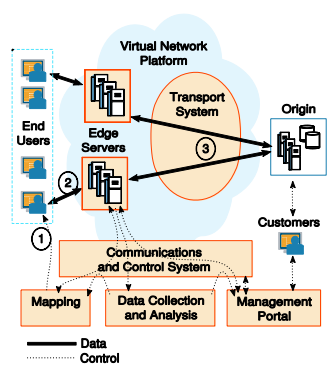
\includegraphics[
        width=0.95\textwidth,
        height=0.65\textheight,
        keepaspectratio
    ]{imagens/cdn-diagram.png}
    
    \vspace{4pt}
    \footnotesize Estrutura lógica simplificada de uma CDN com servidores de origem e de borda.
\end{frame}

\begin{frame}{Monitoramento de Memória}
\textbf{APIs de Sistemas Operacionais}
\begin{itemize}
    \item Kernels mantêm estatísticas detalhadas de memória principal e I/O de disco;
    \item \textbf{Linux}: arquivos como \texttt{/proc/meminfo} e \texttt{/proc/diskstats} e interfaces de \textit{cgroups} \cite{linux_procfs_doc, linux_iostats_doc};
    \item \textbf{Windows} e \textbf{macOS} expõem contadores e APIs específicas \cite{windows_mem_counters, windows_disk_counters, macos_virtmem_doc, macos_iokit_doc};
    \item Fornecem base para medir \textbf{uso de RAM} e \textbf{taxa de leitura de disco} por servidor ou contêiner.
\end{itemize}
\end{frame}

\begin{frame}{Interpretação de Dados Desatualizados}
\begin{itemize}
    \item Em sistemas distribuídos, informações de carga chegam ao balanceador com \textbf{atraso};
    \item Dados desatualizados podem \textbf{sobrecarregar} servidores em vez de evitá-lo \cite{adaptiveLoadSharing1986, analysisDelaysLoadSharing1989};
    \item Alternativas ingênuas: ignorar dados de carga (algoritmos cegos) ou usar apenas um subconjunto aleatório de servidores;
    \item O trabalho \textit{Interpreting Stale Load Information} propõe algoritmos que \textbf{interpretam} a carga em função de sua idade, como o \textbf{Basic LI} \cite{interpretingStaleLoadInformation2000};
    \item Este conceito é adaptado neste TCC para métricas de memória.
    \end{itemize}
\end{frame}

\begin{frame}{Virtualização de Redes e Containers}
\begin{itemize}
    \item \textbf{Virtualização de redes}: múltiplas redes virtuais sobre a mesma infraestrutura física \cite{aSurveyOfNetworkVirtualization2010};
    \item \textbf{Containers Linux}: permitem múltiplos ambientes isolados compartilhando o mesmo kernel;
    \item Ferramentas como \textbf{Docker} e LXC reduzem \textit{overhead} em comparação com VMs completas;
    \item Viabilizam criação de \textbf{ambientes de teste reproduzíveis}, com controle fino sobre recursos (cgroups).
\end{itemize}
\end{frame}

%-------------------------------------------------

\section{Trabalhos Relacionados}

\begin{frame}{Trabalhos Relacionados (Parte 1)}
    \centering
    \scriptsize
    \begin{tabular}{|p{0.22\textwidth}|p{0.35\textwidth}|p{0.35\textwidth}|}
        \hline
        \textbf{Título} & \textbf{Proposta} & \textbf{Limitações} \\
        \hline
        NGINX \cite{nginxAlgorithmsEvaluationYuhong2022, nginxDoc} &
        Algoritmos clássicos de balanceamento HTTP (\textit{Round-Robin}, \textit{Least Connections}, \textit{IP hash}). &
        Não usa métricas de \textbf{memória} e I/O de disco para decisões de roteamento. \\
        \hline
        HAProxy \cite{haproxy} &
        Balanceador TCP/HTTP de alta eficiência e baixo consumo de recursos. &
        Não oferece balanceamento nativo guiado por \textbf{uso de memória} dos servidores. \\
        \hline
        Docker Swarm (memória) \cite{dockerswarmmemory2018} &
        Acrescenta consumo de \textbf{memória} como fator no balanceamento interno do Swarm. &
        Restrito ao Docker; não trata CDNs nem métricas diretas de QoE em vídeo. \\
        \hline
        Algoritmo dinâmico em cloud \cite{novelWeightAssignmentLoadBalancingAlgorithmForCloudApps2023} &
        Usa múltiplas métricas (CPU, memória, largura de banda, etc.) para lidar com \textit{flash crowds}. &
        Focado em aplicações \textbf{cloud} genéricas; não é específico para servidores de conteúdo nem para gargalos de memória. \\
        \hline
    \end{tabular}
\end{frame}

\begin{frame}{Trabalhos Relacionados (Parte 2)}
    \centering
    \scriptsize
    \begin{tabular}{|p{0.22\textwidth}|p{0.35\textwidth}|p{0.35\textwidth}|}
        \hline
        \textbf{Título} & \textbf{Proposta} & \textbf{Limitações} \\
        \hline
        Revisão de algoritmos dinâmicos \cite{webServerPerformanceImprovement2021Review} &
        Compara 15 algoritmos de balanceamento dinâmico para servidores web. &
        Poucos usam memória/disco, e nenhum trata esses recursos como \textbf{parâmetro principal} exclusivo. \\
        \hline
        iSCON para vídeo \cite{dynamicLoadBalancingForEfficientVideoStreamingService2015} &
        Replica vídeos populares e balanceia carga com base na \textbf{largura de banda} de saída. &
        Considera predominantemente banda de rede; ignora gargalos de \textbf{memória} e disco. \\
        \hline
        Servidores de vídeo distrib. \cite{dataAllocationAndDynamicLoadBalancingForDistributedVideoStorageServer1999} &
        Duas fases: alocação inicial de réplicas e \textit{load shifting} por \textbf{streams ativas}. &
        Mede carga apenas por número de streams; ignora uso real de \textbf{memória} e I/O de disco. \\
        \hline
    \end{tabular}
\end{frame}

%-------------------------------------------------

\section{Proposta}

\subsection{Requisitos Tecnológicos e Arquitetura}

\begin{frame}{Requisitos Tecnológicos}
    \textbf{Componentes Principais}
    \begin{itemize}
        \item \textbf{Servidores de Conteúdo}: 8 servidores MPEG-DASH, com capacidades heterogêneas de memória e disco;
        \item \textbf{Balanceador de Carga}: Implementado em \textit{Rust}, responsável por aplicar os algoritmos de seleção de servidor;
        \item \textbf{Cliente Gerador de Carga}: Aplicação em \textit{Python} que simula múltiplos usuários MPEG-DASH concorrentes;
        \item \textbf{Servidor MQTT}: \textit{Broker} NanoMQ utilizado para transporte assíncrono de métricas entre servidores e balanceador.
    \end{itemize}
\end{frame}

\begin{frame}{Arquitetura Geral do Sistema}
    \centering
    
\includegraphics[
        width=0.9\textwidth,
        height=0.7\textheight,
        keepaspectratio
    ]{imagens/arch.png}
    \par
    \vspace{4pt}
    \footnotesize Arquitetura geral do sistema experimental (autor, 2025).
\end{frame}

\subsection{Algoritmo}

\begin{frame}{Objetivo do Algoritmo}
\begin{itemize}
    \item Definir o método de escolha de um servidor para cada nova requisição de vídeo;
    \item Algoritmo de natureza \textbf{probabilística}, baseado no \textbf{Basic Load Interpretation} \cite{interpretingStaleLoadInformation2000};
    \item Probabilidade de escolha de cada servidor ajustada dinamicamente de acordo com:
    \begin{itemize}
        \item Consumo de \textbf{memória RAM};
        \item Taxa de entrada e saída de \textbf{disco} (I/O);
        \item \textbf{Idade} das informações de carga.
    \end{itemize}
    \item Servidores publicam periodicamente suas métricas de carga para o balanceador.
\end{itemize}
\end{frame}

\begin{frame}{Cálculo da Probabilidade}
A probabilidade ($P_i$) de uma requisição ser enviada para um servidor $i$ é baseada no \textbf{Basic Load Interpretation}:

\begin{equation}\label{eq:basic_li}
    P_{i}=\frac{\frac{L_{tot}+arrive_{T}}{n}-L_{i}}{arrive_{T}}
\end{equation}

\begin{itemize}
    \item[$P_i$]: Probabilidade de escolha do servidor $i$;
    \item[$n$]: Número total de servidores disponíveis;
    \item[$L_i$]: Carga individual reportada pelo servidor $i$;
    \item[$L_{tot}$]: Somatório de todas as cargas reportadas ($\sum L_i$);
    \item[$arrive_T$]: Número esperado de novas requisições durante o intervalo médio $T$ das informações de carga.
\end{itemize}
\end{frame}

\begin{frame}{Cálculo de $arrive_T$}
O parâmetro $arrive_T$ representa o número esperado de requisições durante o intervalo de desatualização:

\begin{equation}\label{eq:arrive_t}
arrive_T = \left( \frac{R_{total}}{T_{elapsed}} \right) \cdot T_{stale} \cdot \left( \frac{L_{tot}}{R_{active}} \right) \cdot C
\end{equation}

\begin{itemize}
    \item[$R_{total}$]: Total de requisições recebidas pelo balanceador;
    \item[$T_{elapsed}$]: Tempo total de execução do balanceador;
    \item[$T_{stale}$]: Tempo médio de desatualização das métricas;
    \item[$R_{active}$]: Requisições ativas ($\sum_{i=1}^{n} AR_i$);
    \item[$C$]: Constante de ajuste (definida heuristicamente).
\end{itemize}
\end{frame}

\begin{frame}{Adaptação do Parâmetro de Carga ($L_i$)}
No contexto deste trabalho, a \textbf{carga} ($L_i$) é medida a partir do uso de memória:

\begin{equation}\label{eq:limemory}
    L_i = CM \cdot LM_i + CD \cdot LD_i
\end{equation}

\begin{itemize}
    \item[$LM_i$]: Consumo de \textbf{memória} normalizado do servidor $i$ (0--1);
    \item[$LD_i$]: Carga de \textbf{disco} (I/O) normalizada do servidor $i$ (0--1);
    \item[$CM, CD$]: Coeficientes dinâmicos que refletem a importância relativa de memória e disco.
\end{itemize}
\end{frame}

\begin{frame}{Cálculo dos Coeficientes Dinâmicos ($CM$ e $CD$)}
Os coeficientes aumentam o peso do recurso mais pressionado no sistema como um todo.

\begin{itemize}
    \item Taxa média de uso de memória:
    \[
        TM = \frac{1}{n}\sum_{i=1}^n LM_i
    \]
    \item Taxa média de uso de disco:
    \[
        TD = \frac{1}{n}\sum_{i=1}^n LD_i
    \]
\end{itemize}

\begin{minipage}{.48\textwidth}
    \begin{equation}
        CM = \frac{TM}{TM + TD} \label{eq:cm}
    \end{equation}
\end{minipage}
\hfill
\begin{minipage}{.48\textwidth}
    \begin{equation}
        CD = \frac{TD}{TM + TD} \label{eq:cd}
    \end{equation}
\end{minipage}
\end{frame}

\begin{frame}{Pseudocódigo — Atualização da Distribuição}
    \vspace{-0.5cm}
    \tiny
    \begin{algorithm}[H]
    \caption{Atualização da distribuição de probabilidade}
    \begin{algorithmic}[1]
    \Statex \textbf{Gatilho}: Nova informação de carga via MQTT.
    \Require Métricas $LM_i, LD_i, T_i, AR_i$ para cada servidor $S_i$
    \Ensure Probabilidades $P_i$ atualizadas
    \Procedure{AtualizarDistribuicao}{$LM_i, LD_i, T_i, AR_i$}
        \State Atualizar métricas do servidor $S_i$
        \State $TM \leftarrow \frac{1}{n} \sum_{i=1}^{n} LM_i$, \quad $TD \leftarrow \frac{1}{n} \sum_{i=1}^{n} LD_i$
        \State $T \leftarrow \frac{1}{n} \sum_{i=1}^{n} (T_{atual} - T_i)$
        \State Calcular $CM$ e $CD$ (Eq. \ref{eq:cm}, \ref{eq:cd})
        \State Calcular $L_i$ para cada servidor (Eq. \ref{eq:limemory})
        \State $L_{tot} \leftarrow \sum_{i=1}^{n} L_i$
        \State Calcular $arrive_T$ (Eq. \ref{eq:arrive_t})
        \State Calcular $P_i$ para cada servidor (Eq. \ref{eq:basic_li})
        \If{$n = 0$ \textbf{ou} $arrive_T \leq 0$}
            \State $P_i \leftarrow 1/n$ para todos os servidores
        \EndIf
    \EndProcedure
    \end{algorithmic}
    \end{algorithm}
\end{frame}

%-------------------------------------------------

\section{Implementação}

\begin{frame}{Ambiente Experimental}
    \begin{itemize}
        \item Ambiente executado em uma única máquina física (\textbf{Windows} + \textbf{WSL2} com kernel Linux completo);
        \item Todos os componentes são executados em contêineres \textbf{Docker};
        \item Uso de \textbf{cgroups v2} para monitorar e limitar recursos (memória, I/O de disco);
        \item Limpeza do \textit{page cache} antes de cada bateria de testes para garantir reprodutibilidade.
    \end{itemize}
\end{frame}

\begin{frame}{Organização do Conteúdo e Bind Mounts}
    \begin{itemize}
        \item Conteúdo de vídeo armazenado em \texttt{/data} no \textit{host} WSL, com diretórios específicos para cada servidor:
        \begin{itemize}
            \item \texttt{/data/server-1}, \texttt{/data/server-2}, \dots, \texttt{/data/server-8};
        \end{itemize}
        \item Cada servidor MPEG-DASH monta seu diretório via \textbf{bind mount} Docker;
        \item Simula cenário real de CDNs com \textbf{conteúdo exclusivo} por servidor de borda;
        \item Evita cópia de arquivos para dentro das imagens, reduzindo tamanho e facilitando atualização.
    \end{itemize}
\end{frame}

\begin{frame}{Módulos Principais e Auxiliares}
    \textbf{Módulos Principais}
    \begin{itemize}
        \item \textbf{Servidores MPEG-DASH} (\textit{ASP.NET Core}): servem segmentos de vídeo e publicam métricas de recursos;
        \item \textbf{Balanceador de Carga} (\textit{Rust}): \textit{proxy} reverso HTTP com estratégias \textit{Round-Robin}, Aleatória e Monitoramento de Memória;
        \item \textbf{Gerador de Carga} (\textit{Python}/\texttt{aiohttp}): simula múltiplos clientes concorrentes.
    \end{itemize}

    \vspace{8pt}
    \textbf{Módulos Auxiliares}
    \begin{itemize}
        \item \textbf{\textit{Broker} MQTT (NanoMQ)};
        \item \textbf{Coletor de Métricas} (API em Python);
        \item \textbf{Painel de Monitoramento} em tempo real (HTML + \texttt{Chart.js});
        \item \textbf{Cliente de Validação} MPEG-DASH (\texttt{dash.js}).
    \end{itemize}
\end{frame}

\begin{frame}{Monitoramento e Publicação de Métricas}
    \begin{itemize}
        \item Servidores MPEG-DASH executam um serviço de fundo \texttt{MetricsPublisher};
        \item Leituras periódicas de:
        \begin{itemize}
            \item \texttt{/sys/fs/cgroup/memory.current} (memória utilizada);
            \item \texttt{/sys/fs/cgroup/io.stat} (bytes lidos de disco);
        \end{itemize}
        \item Métricas são normalizadas em relação aos limites configurados para cada contêiner;
        \item Publicação em tópicos MQTT específicos, consumidos pelo balanceador de carga;
        \item Intervalo de publicação configurável (por exemplo, 6s e 30s) para avaliar impacto de dados desatualizados.
    \end{itemize}
\end{frame}

\begin{frame}{Geração de Conteúdo MPEG-DASH}
    \begin{itemize}
        \item Conteúdo gerado com \texttt{ffmpeg}, a partir de um vídeo de referência;
        \item Criação de múltiplas representações (1080p, 720p, 480p, 360p, 240p, 144p);
        \item Segmentação em blocos MPEG-DASH e geração de manifestos MPD;
        \item Conteúdo é replicado para os diretórios de cada servidor, preservando estrutura;
        \item Permite avaliar impacto do balanceamento na \textbf{qualidade adaptativa} do vídeo.
    \end{itemize}
\end{frame}

\begin{frame}{Painel de Monitoramento em Tempo Real}
    \centering
    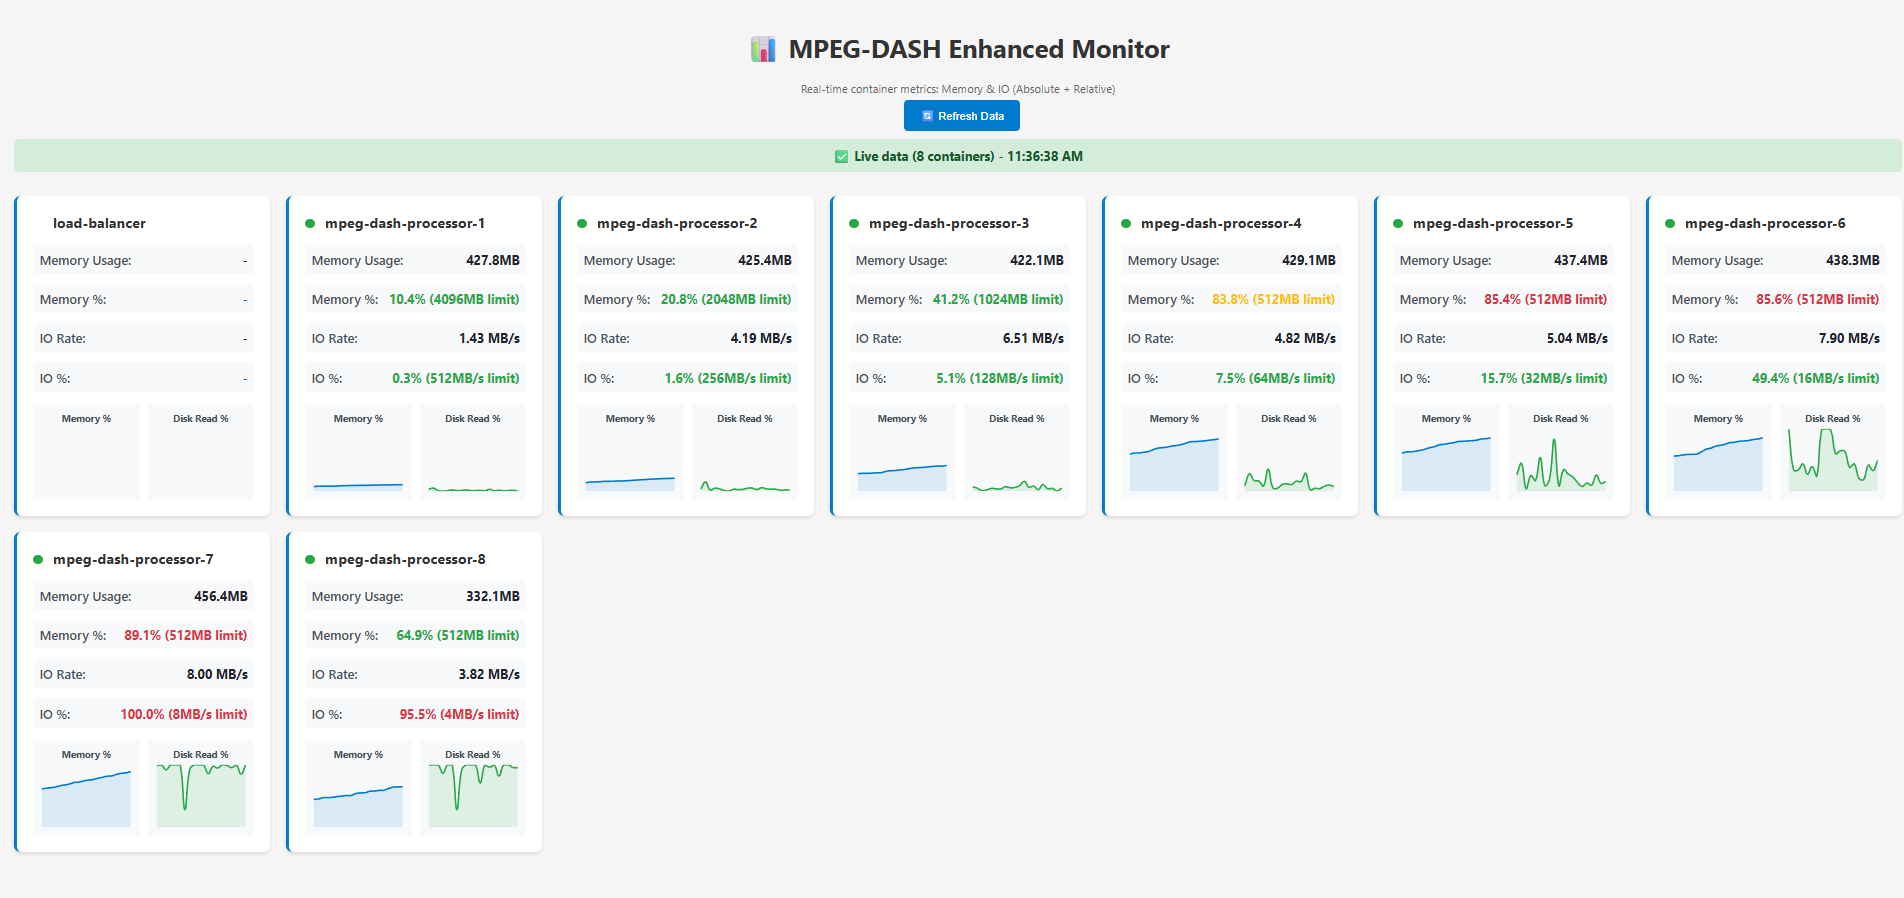
\includegraphics[
        width=0.95\textwidth,
        height=0.7\textheight,
        keepaspectratio
    ]{imagens/mpeg-dash-servers-monitoring.png}
    
    \vspace{4pt}
    \footnotesize Painel de monitoramento em tempo real com métricas de memória, I/O de disco e requisições ativas.
\end{frame}

\begin{frame}{Cliente MPEG-DASH para Validação}
    \centering
    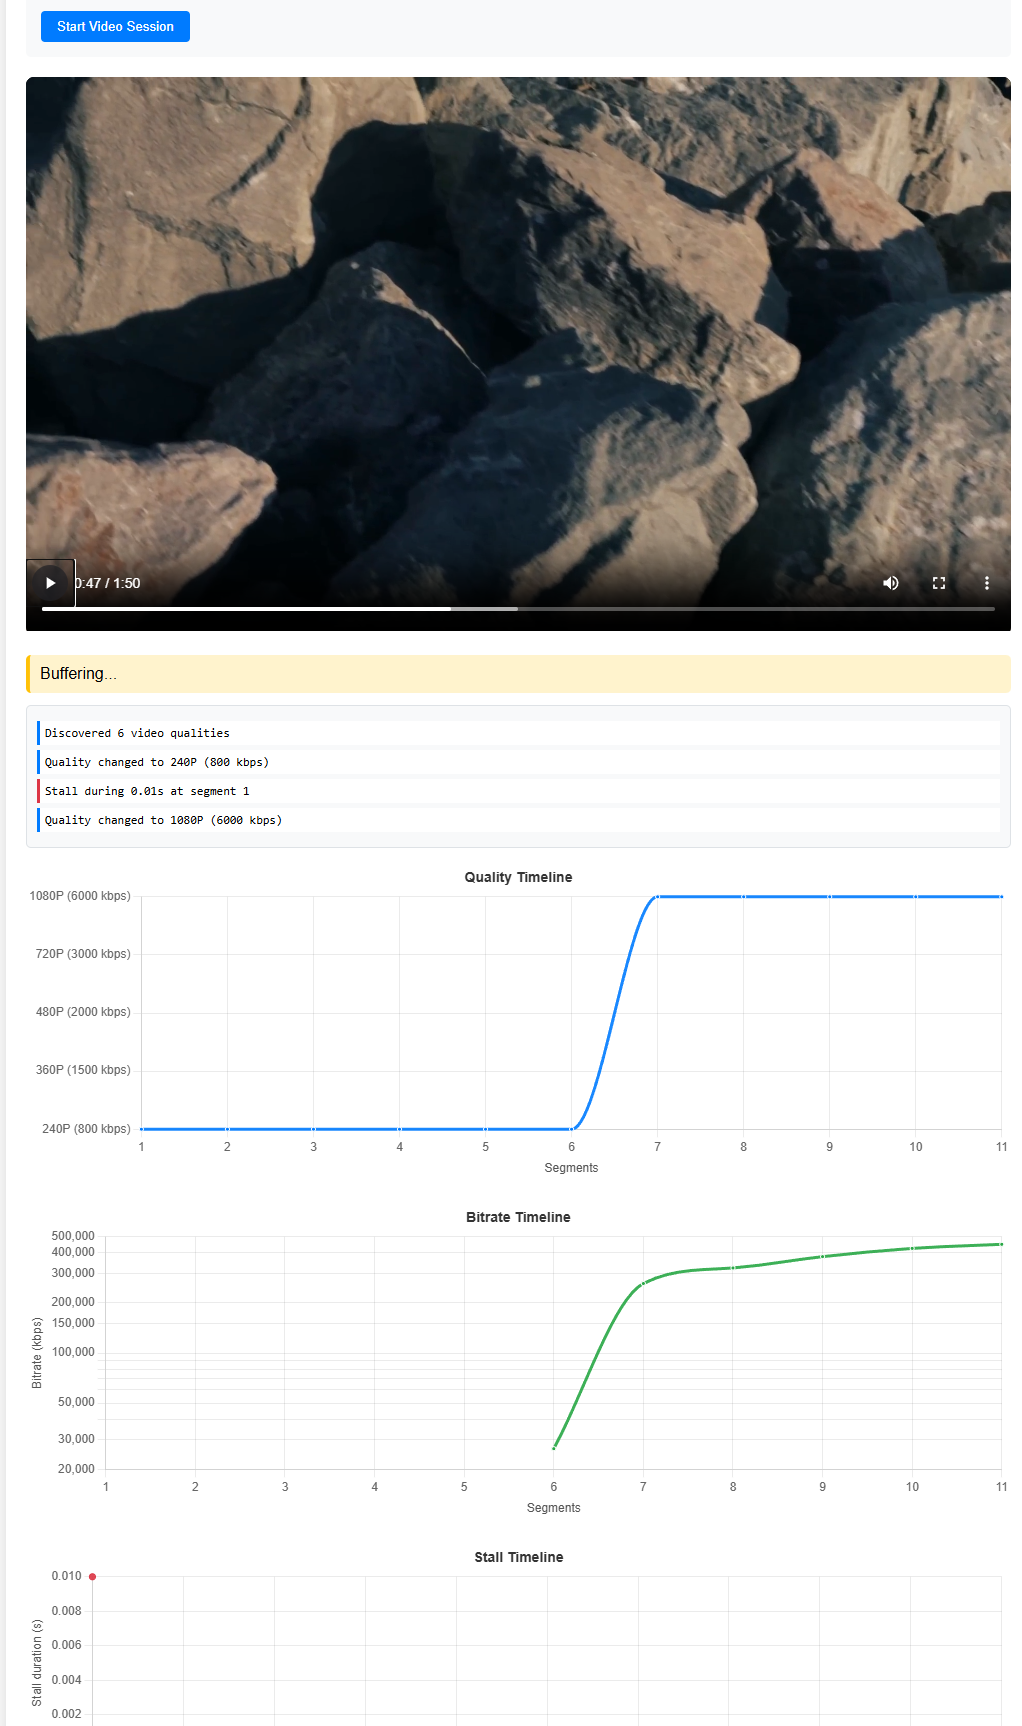
\includegraphics[
        width=0.95\textwidth,
        height=0.7\textheight,
        keepaspectratio
    ]{imagens/mpeg-dash-client-charts-and-video.png}
    
    \vspace{4pt}
    \footnotesize Cliente MPEG-DASH (\texttt{dash.js}) com gráficos em tempo real de qualidade, \textit{bitrate} e travamentos (\textit{stalls}).
\end{frame}

%-------------------------------------------------

\section{Experimentos e Resultados}

\begin{frame}{Cenários de Teste}
    \centering
    \scriptsize
    \begin{tabular}{|c|c|c|p{5.5cm}|}
        \hline
        \textbf{Cenário} & \textbf{Usuários} & \textbf{Distribuição} & \textbf{Configuração dos Servidores} \\
        \hline
        1 & 100 & Heterogênea & 
        \textbf{S1}: 4096MB / 1024MB/s; \textbf{S2}: 2048MB / 512MB/s; \textbf{S3}: 1024MB / 256MB/s; \textbf{S4}: 512MB / 128MB/s; \textbf{S5}: 256MB / 64MB/s; \textbf{S6}: 128MB / 32MB/s; \textbf{S7}: 64MB / 16MB/s; \textbf{S8}: 32MB / 8MB/s \\
        \hline
        2 & 100 & Homogênea & 
        Todos os servidores: 1024MB RAM e 256MB/s de leitura \\
        \hline
        3 & 1000 & Heterogênea & 
        Mesma configuração do Cenário 1 \\
        \hline
        4 & 1000 & Homogênea & 
        Mesma configuração do Cenário 2 \\
        \hline
    \end{tabular}
\end{frame}

\begin{frame}{Estratégias de Balanceamento}
    \begin{itemize}
        \item \textbf{\textit{Round-Robin}}: distribuição cíclica uniforme;
        \item \textbf{Seleção Aleatória}: servidor escolhido de forma uniforme e aleatória a cada requisição;
        \item \textbf{Monitoramento de Memória (6s)}: algoritmo proposto com atualização frequente de métricas;
        \item \textbf{Monitoramento de Memória (30s)}: algoritmo proposto com dados moderadamente desatualizados.
    \end{itemize}
\end{frame}

\begin{frame}{Métricas de Avaliação de QoE}
    \begin{itemize}
        \item \textbf{Latência Média} de resposta por requisição HTTP;
        \item \textbf{Qualidade} de vídeo ao longo da sessão (resoluções escolhidas pelo cliente);
        \item \textbf{\textit{Bitrate}} médio por segmento;
        \item \textbf{Travamentos} (\textit{stalls}): quantidade, duração total e maior duração.
    \end{itemize}
\end{frame}

\begin{frame}{Qualidade de Vídeo por Cenário}
    \centering
    \begin{tabular}{@{}cc@{}}
        
\includegraphics[width=0.5\textwidth]{imagens/outputs/quality-charts/scenario-1.png} &
        
\includegraphics[width=0.5\textwidth]{imagens/outputs/quality-charts/scenario-2.png} \\
        
\includegraphics[width=0.5\textwidth]{imagens/outputs/quality-charts/scenario-3.png} &
        
\includegraphics[width=0.5\textwidth]{imagens/outputs/quality-charts/scenario-4.png}
    \end{tabular}
\end{frame}

\begin{frame}{Bitrate por Cenário}
    \centering
    \begin{tabular}{@{}cc@{}}
        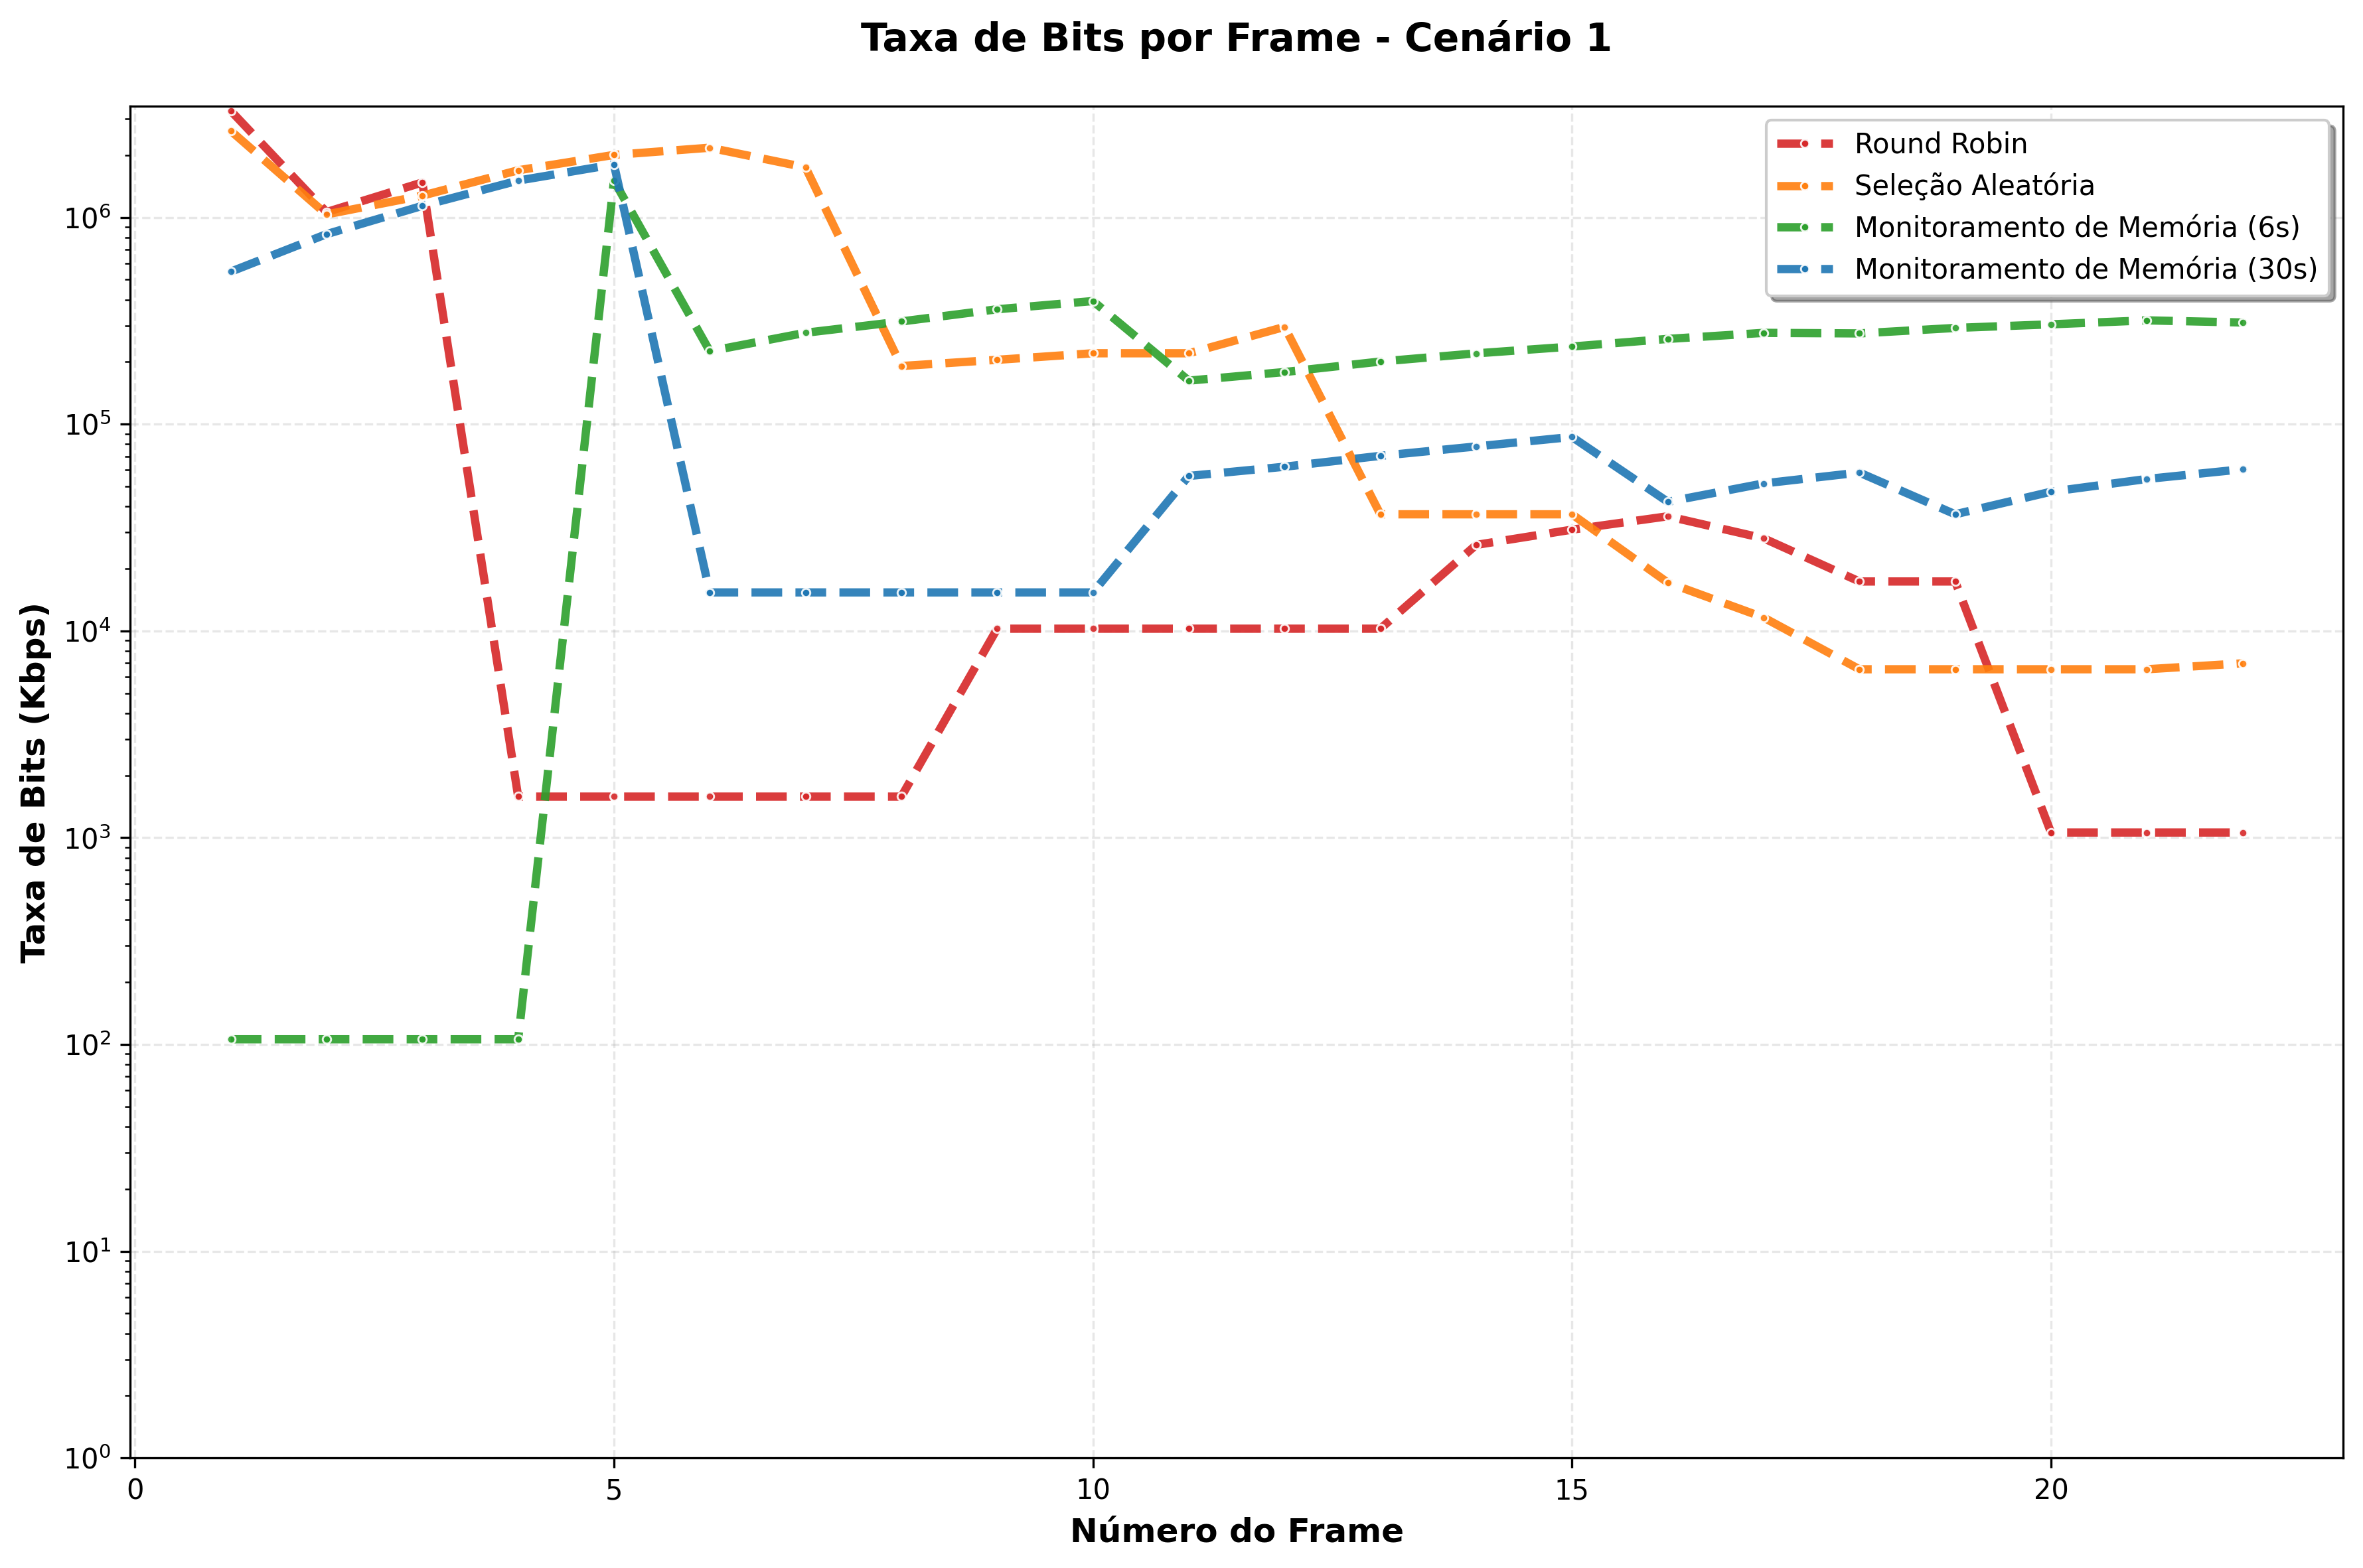
\includegraphics[width=0.5\textwidth]{imagens/outputs/bitrate-charts/scenario-1.png} &
        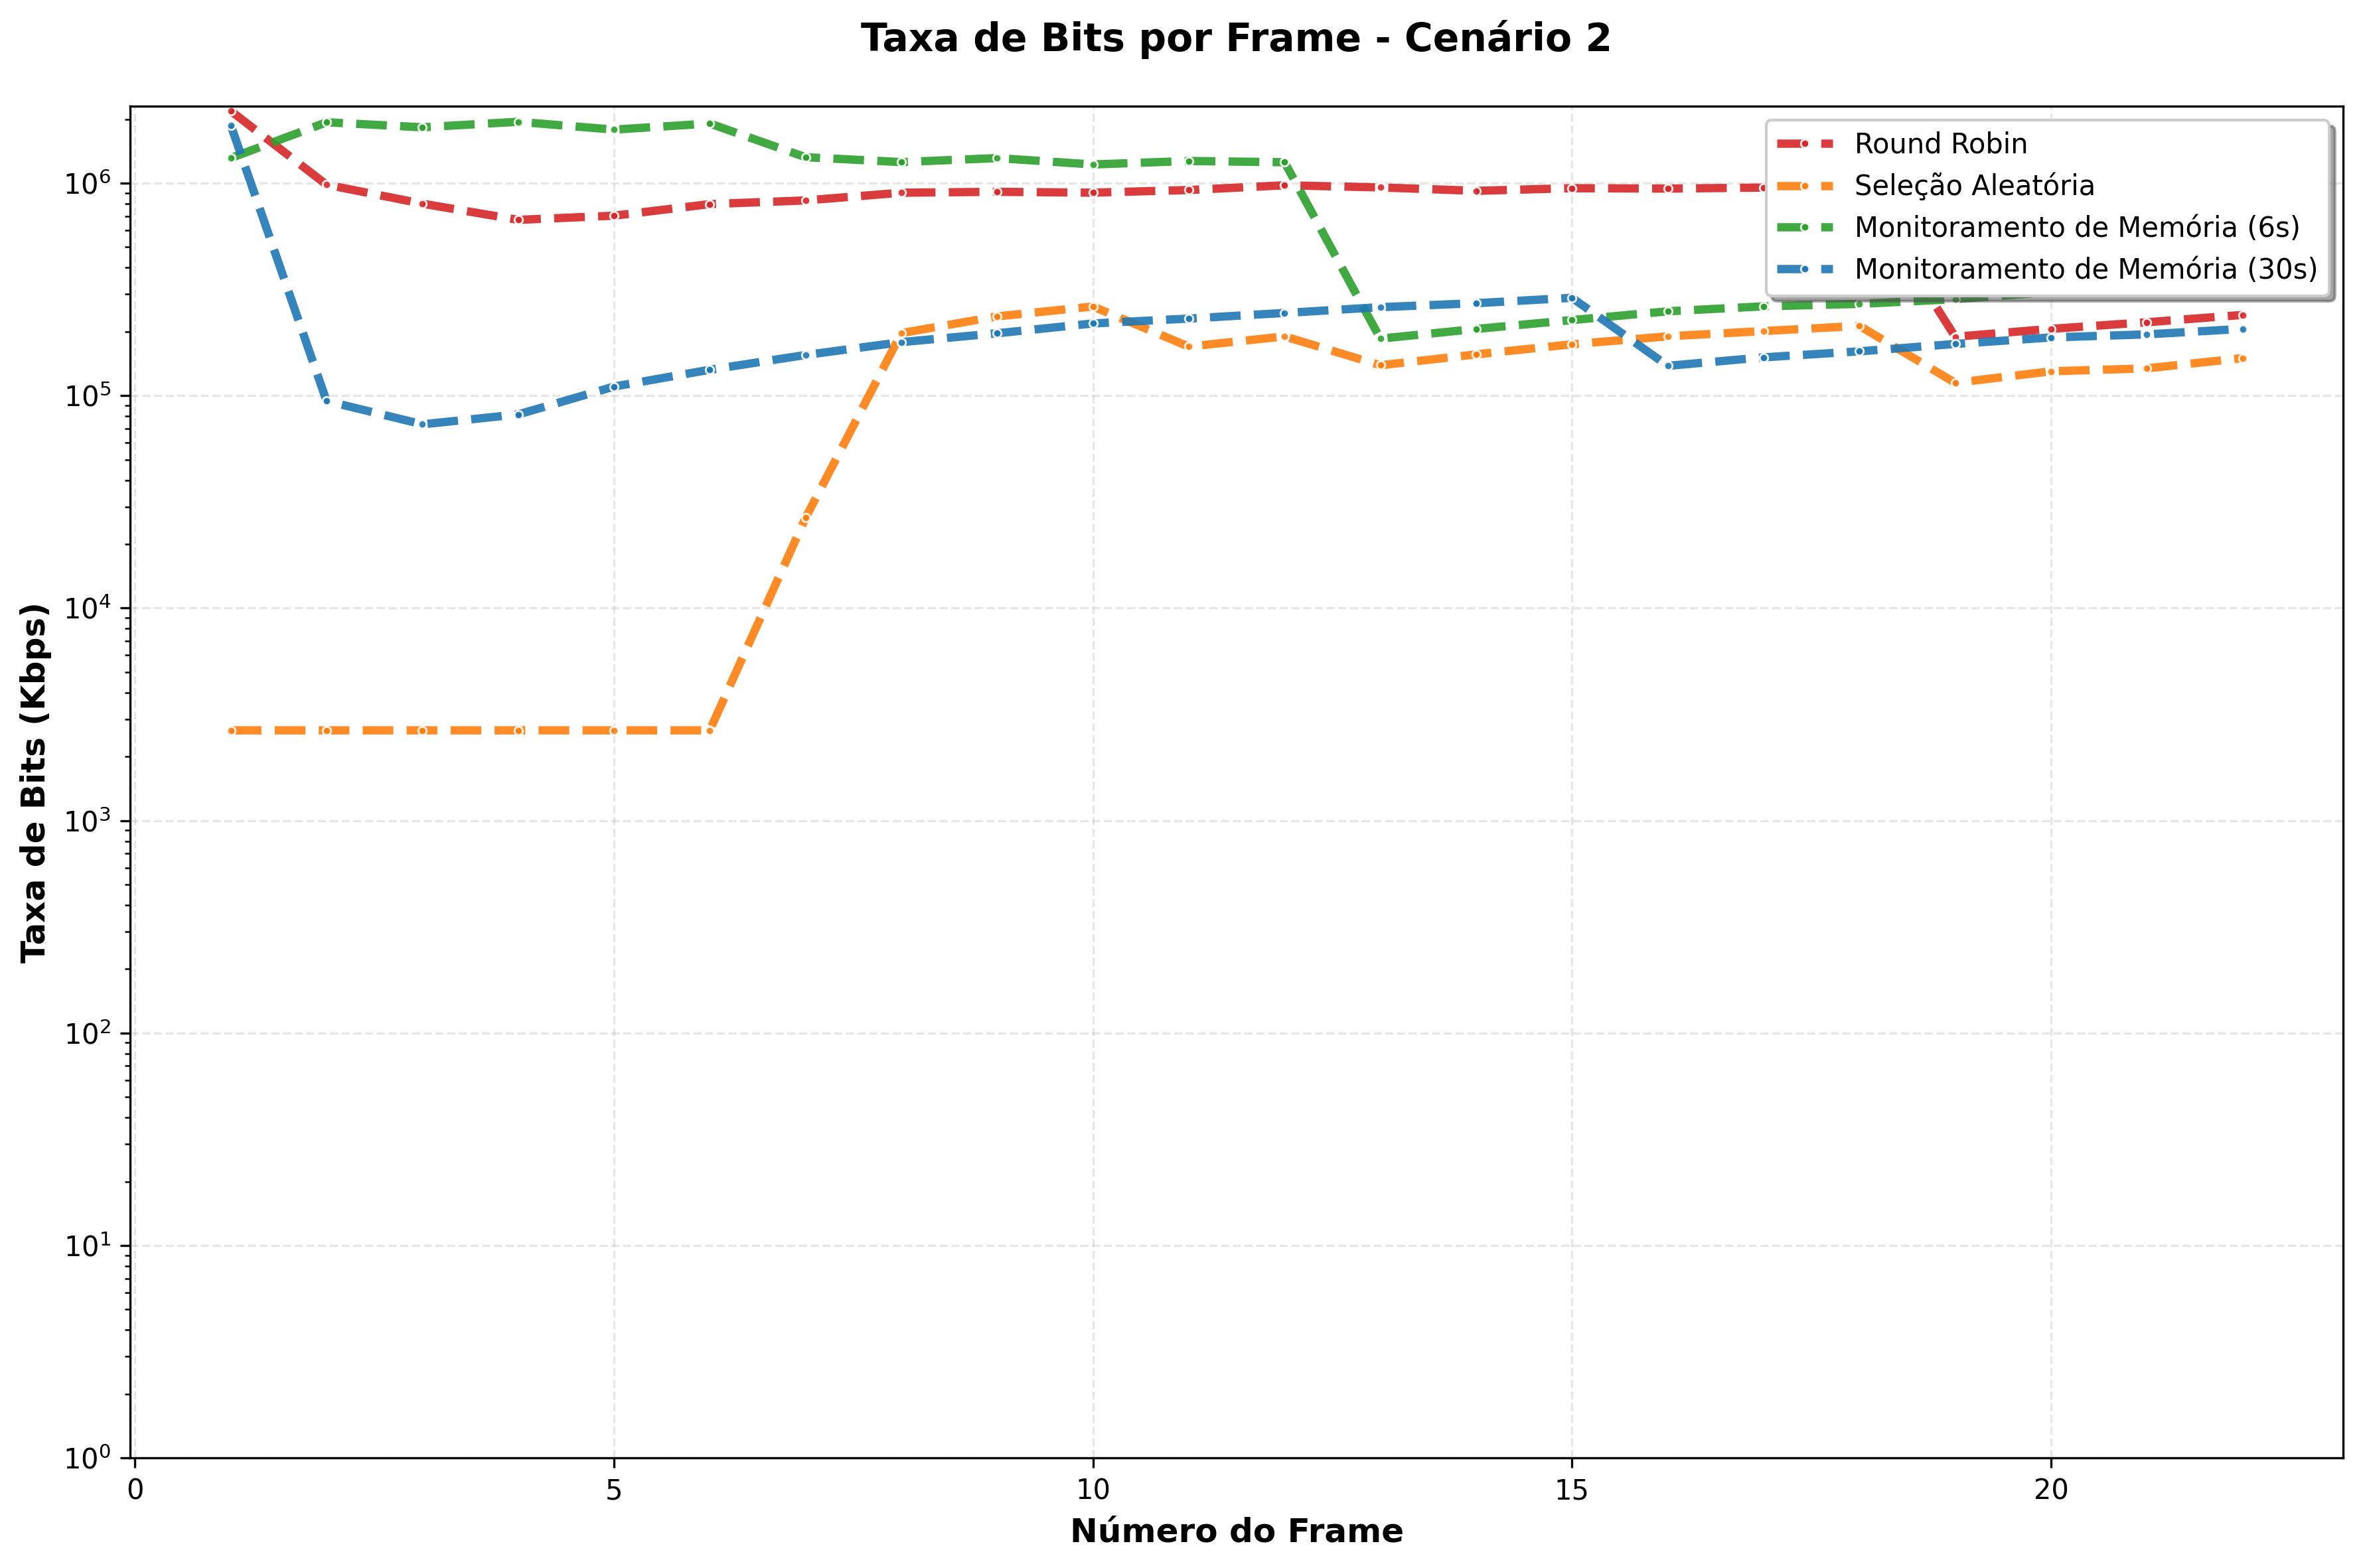
\includegraphics[width=0.5\textwidth]{imagens/outputs/bitrate-charts/scenario-2.png} \\
        
\includegraphics[width=0.5\textwidth]{imagens/outputs/bitrate-charts/scenario-3.png} &
        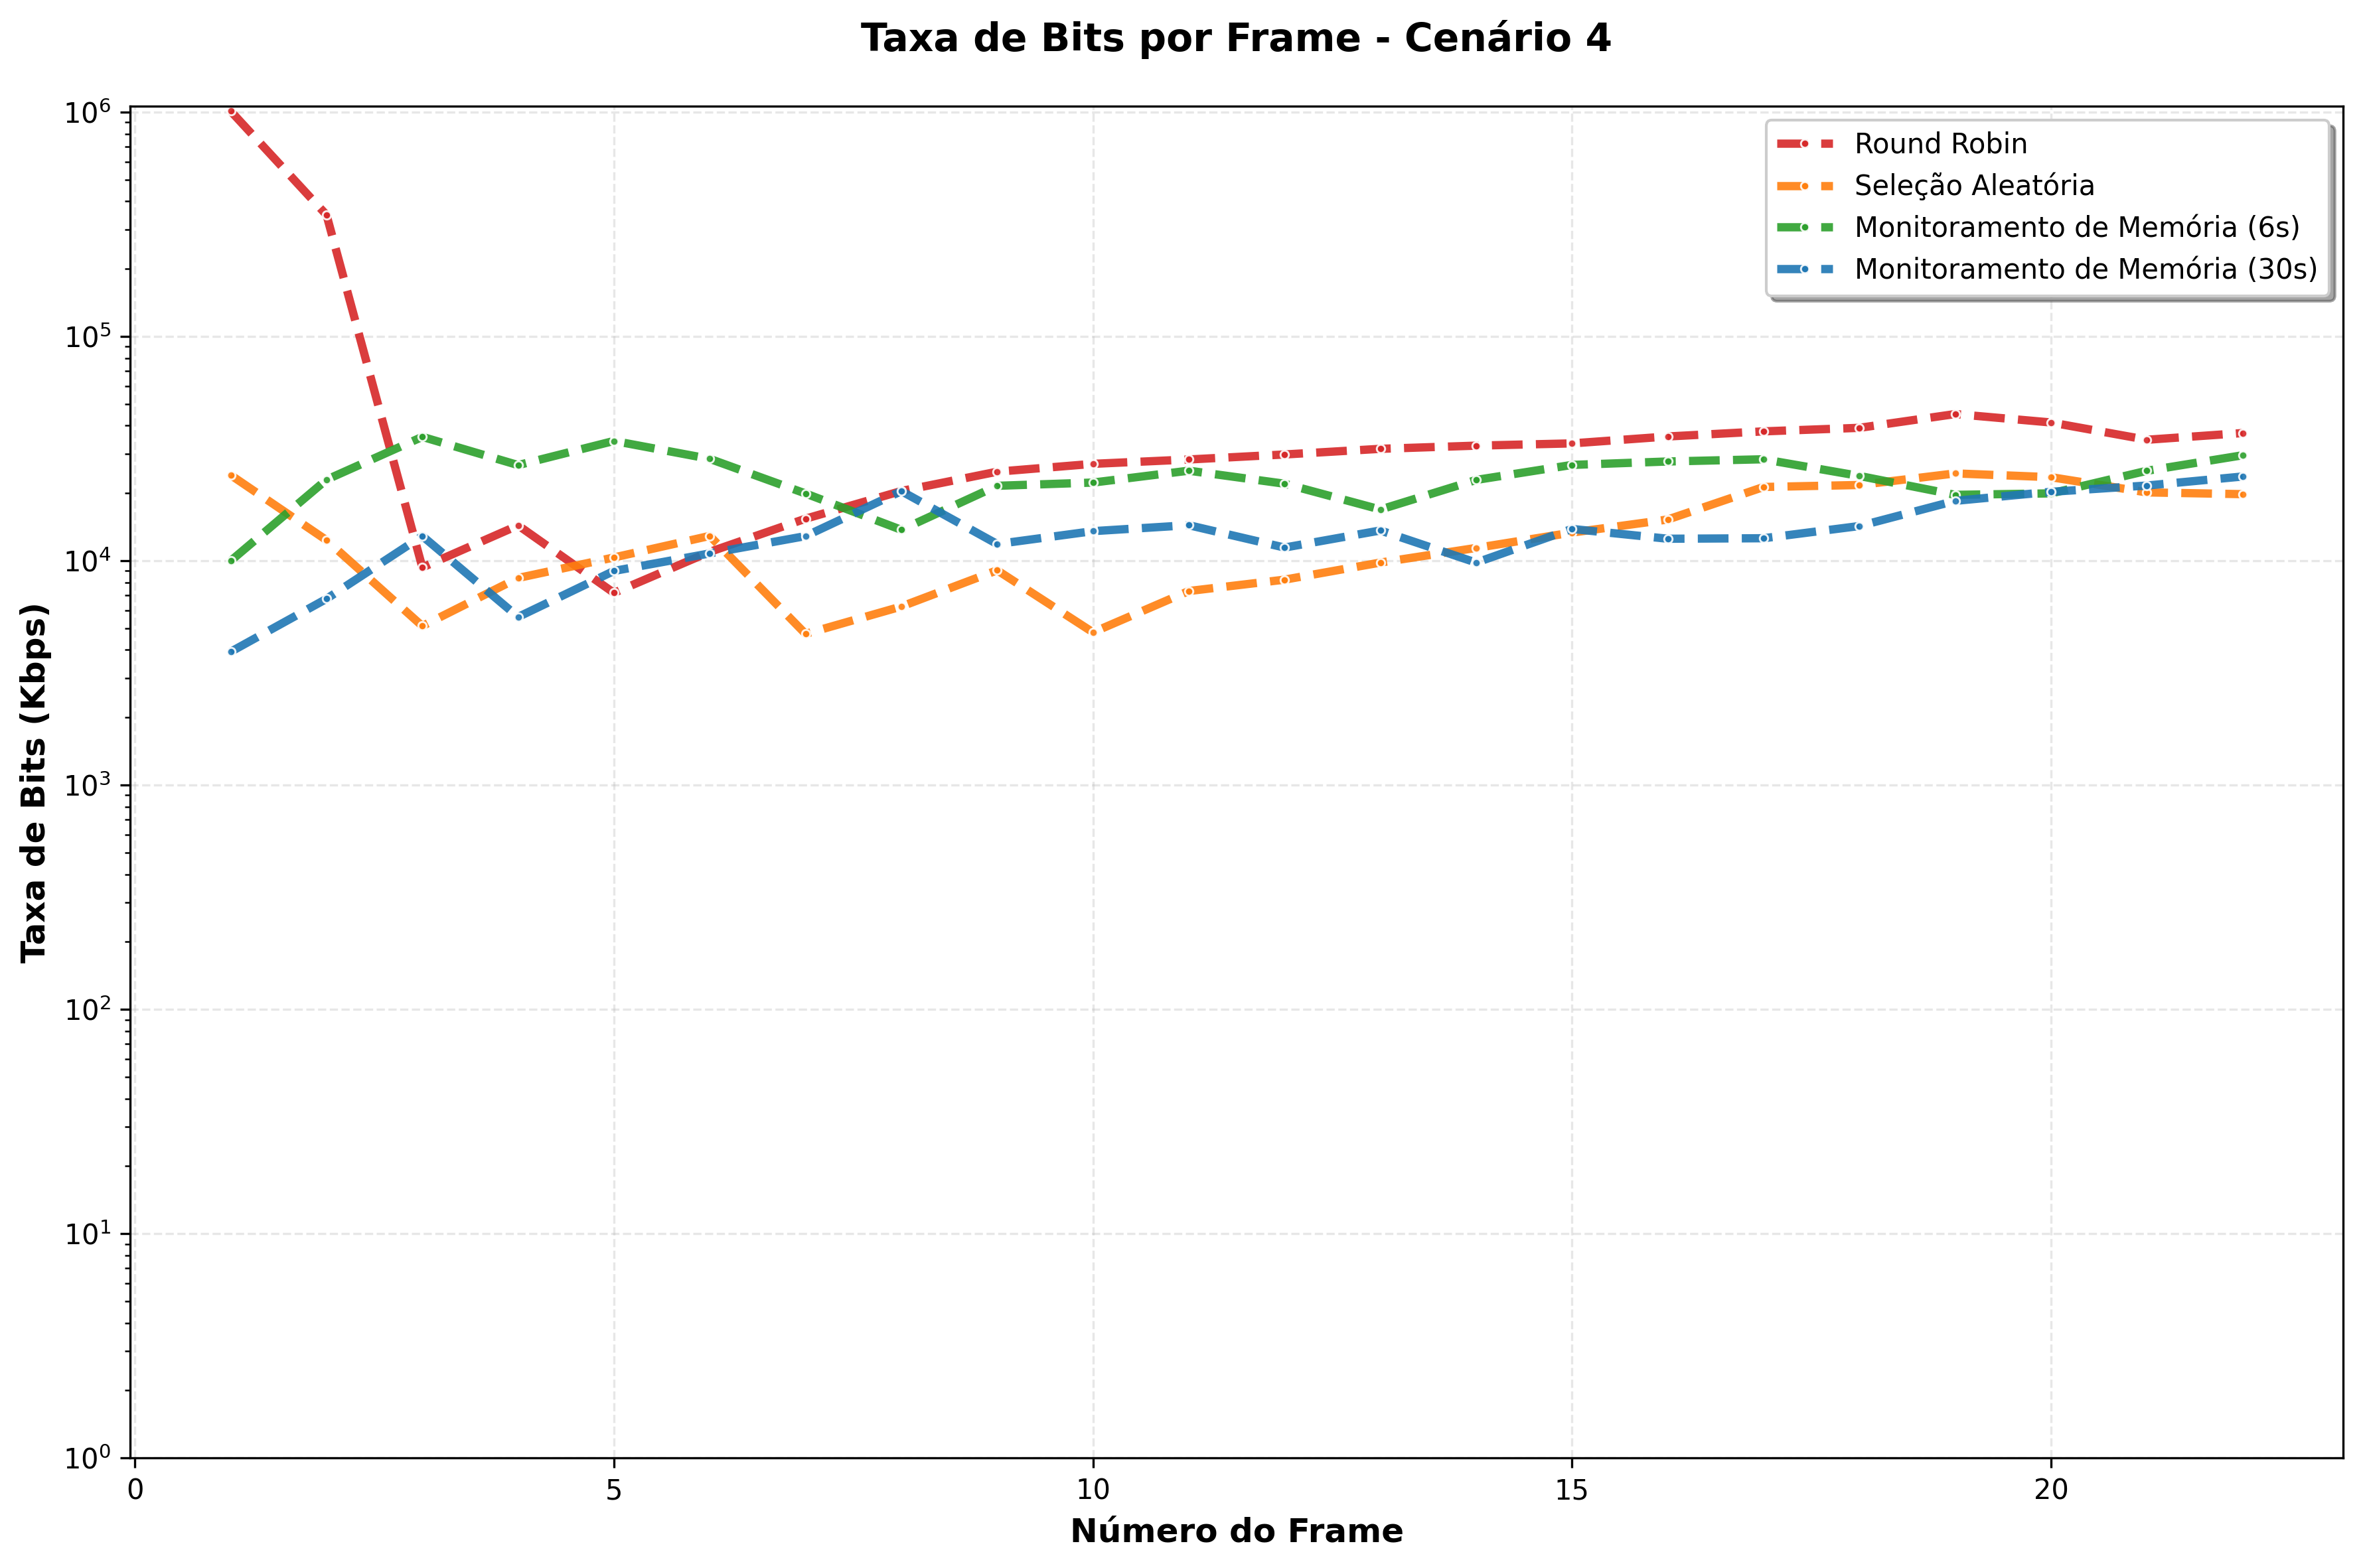
\includegraphics[width=0.5\textwidth]{imagens/outputs/bitrate-charts/scenario-4.png}
    \end{tabular}
\end{frame}

\begin{frame}{Stalls por Cenário}
    \centering
    \begin{tabular}{@{}cc@{}}
        
\includegraphics[width=0.5\textwidth]{imagens/outputs/stall-charts/scenario-1.png} &
        
\includegraphics[width=0.5\textwidth]{imagens/outputs/stall-charts/scenario-2.png} \\
        
\includegraphics[width=0.5\textwidth]{imagens/outputs/stall-charts/scenario-3.png} &
        
\includegraphics[width=0.5\textwidth]{imagens/outputs/stall-charts/scenario-4.png}
    \end{tabular}
\end{frame}

\begin{frame}{Latência Média por Cenário}
    \centering
    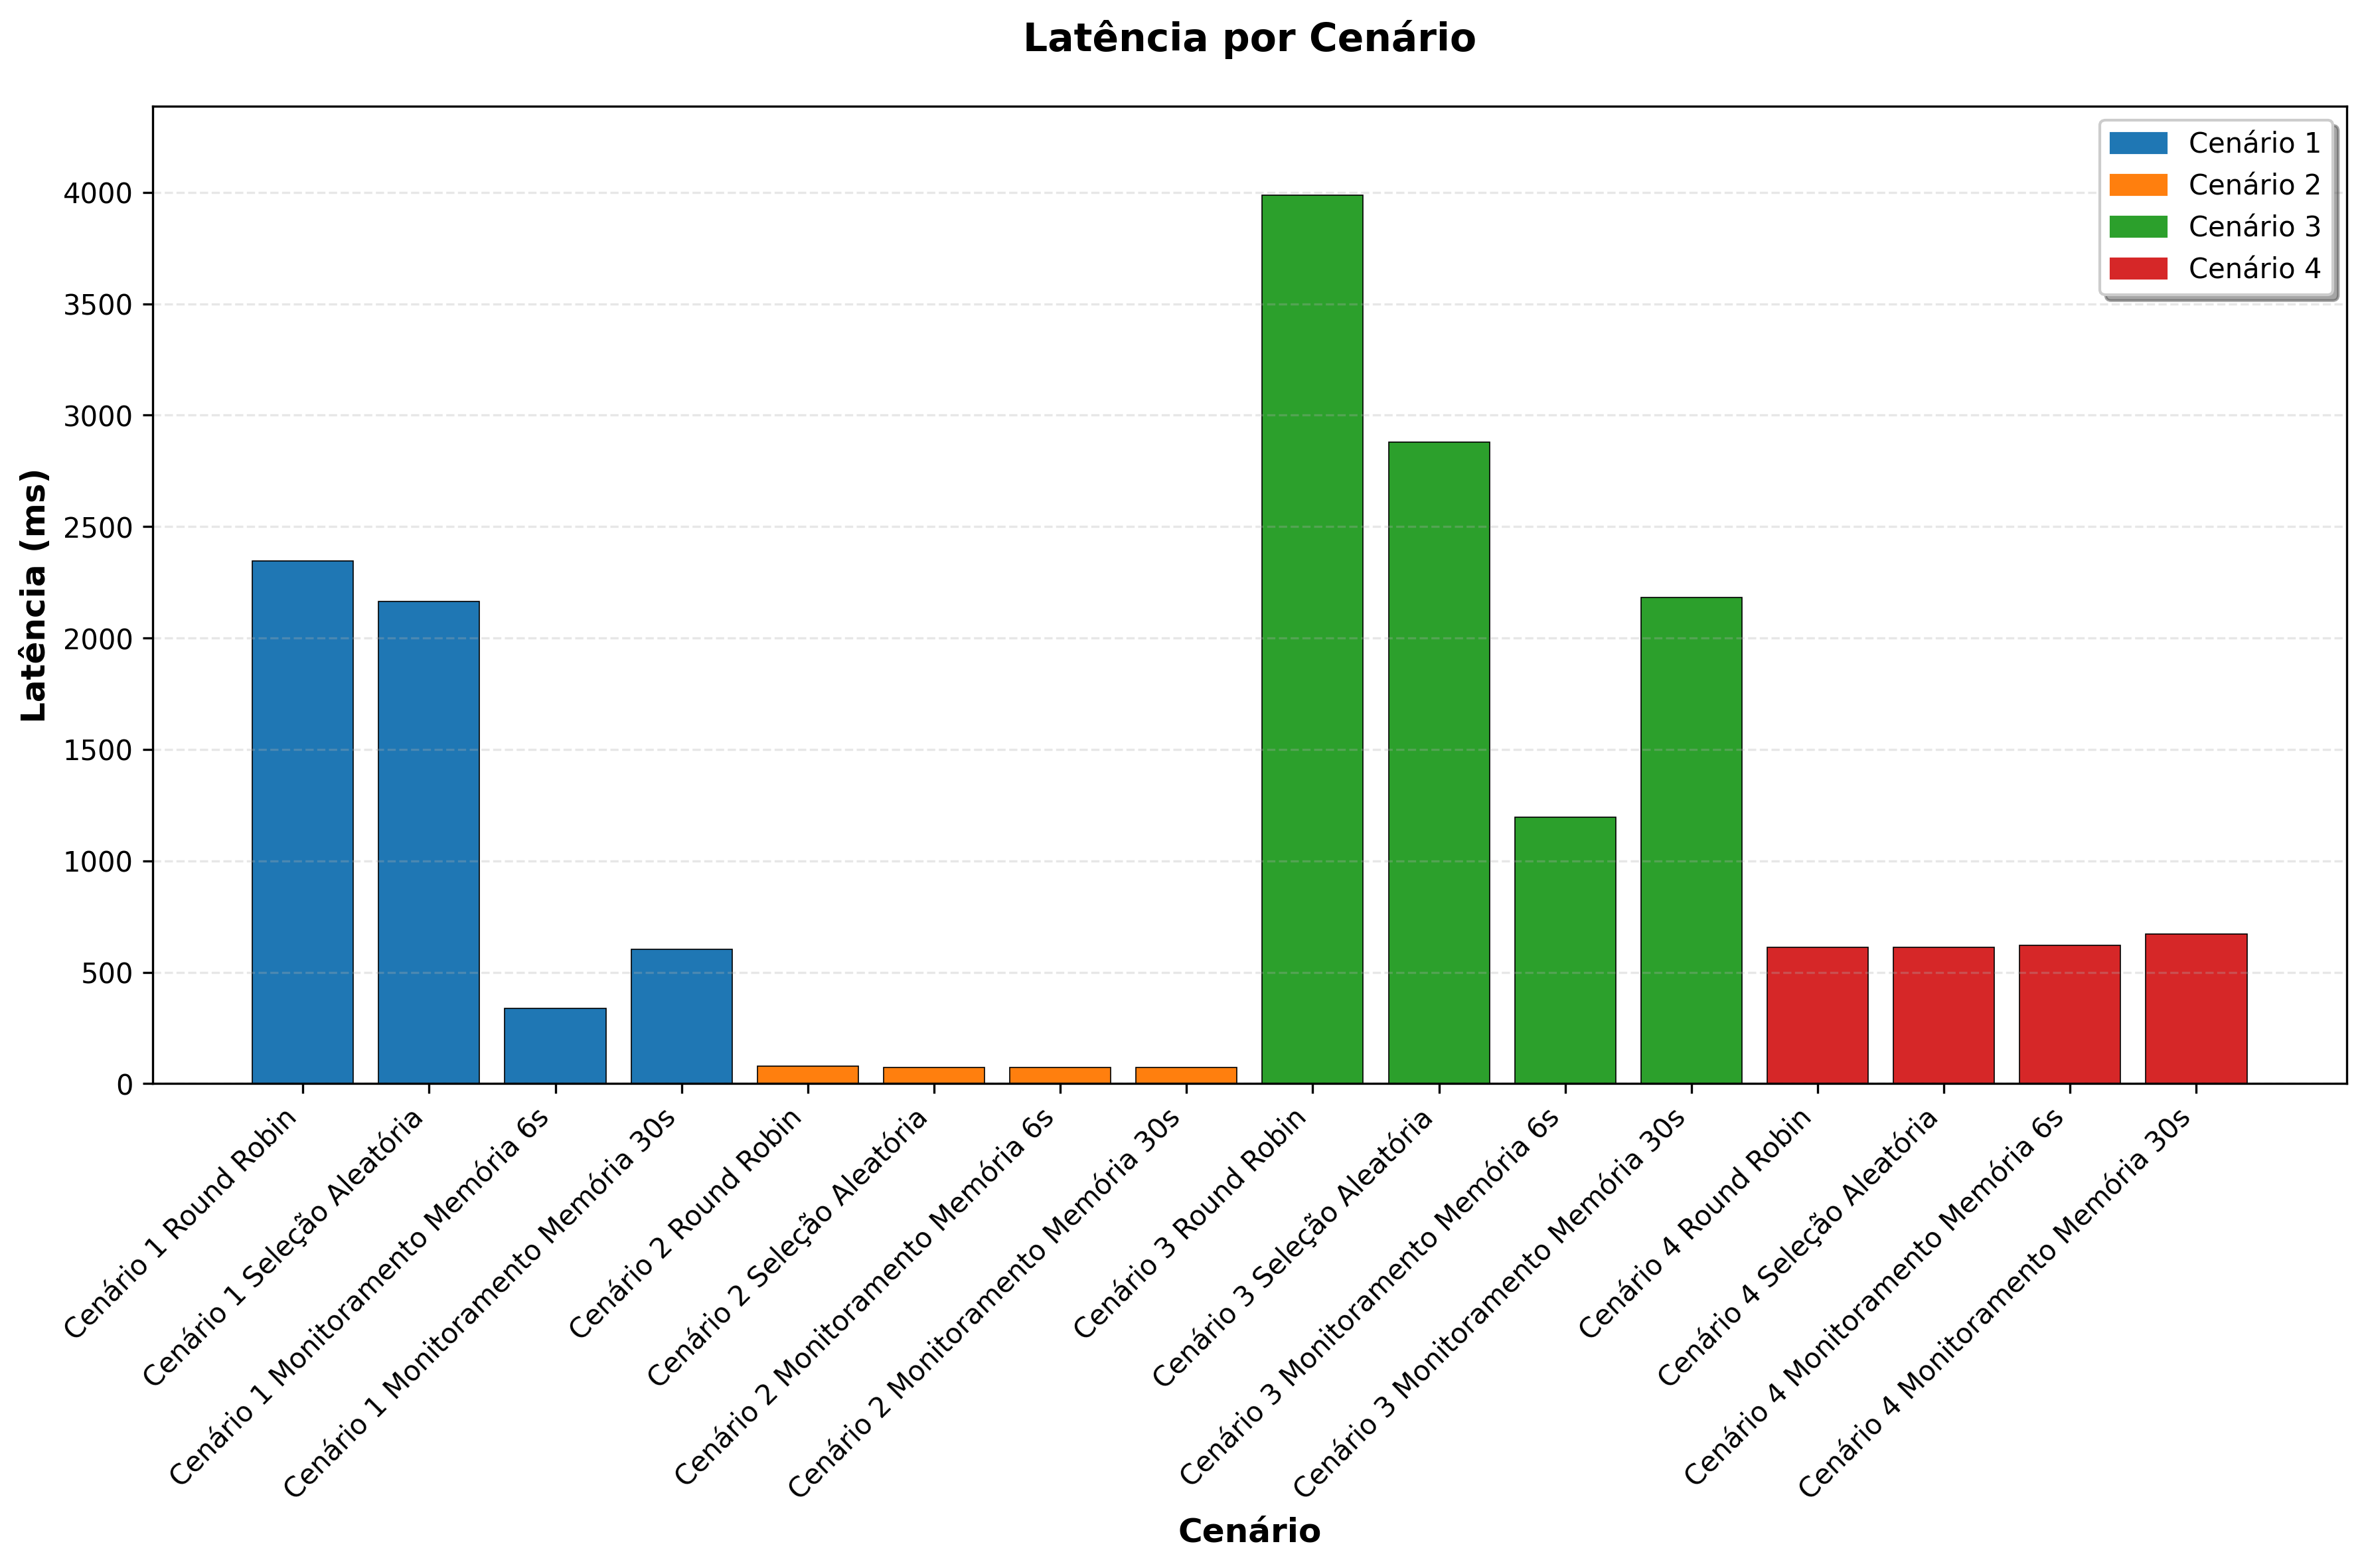
\includegraphics[
        width=0.85\textwidth,
        keepaspectratio
    ]{imagens/outputs/latency_chart.png}
    
    \vspace{4pt}
    \footnotesize Latência média de resposta por cenário e estratégia de balanceamento.
\end{frame}

\begin{frame}{Síntese dos Resultados}
    \begin{itemize}
        \item Em cenários \textbf{heterogêneos} (1 e 3), o algoritmo proposto (\textbf{MM 6s}) reduziu a latência média em até \textbf{85,7\%} em relação ao \textit{Round-Robin};
        \item No Cenário 3, estratégias clássicas apresentaram múltiplos travamentos e queda de qualidade para 144p, enquanto o algoritmo proposto eliminou travamentos e manteve qualidade alta (720p--1080p);
        \item A variante com \textbf{30s} de atualização, mesmo com dados desatualizados, superou consistentemente as estratégias clássicas;
        \item Em cenários \textbf{homogêneos} (2 e 4), todas as estratégias apresentaram desempenho similar, evidenciando que o benefício do algoritmo está ligado à heterogeneidade.
    \end{itemize}
\end{frame}

%-------------------------------------------------

\section{Conclusão}

\begin{frame}{Validação das Hipóteses}
    \begin{itemize}
        \item \textbf{Hipótese 1}: Algoritmo baseado em monitoramento de memória supera \textit{Round-Robin} e Aleatório em ambientes heterogêneos:
        \begin{itemize}
            \item Confirmada por reduções expressivas de latência e eliminação de travamentos.
        \end{itemize}
        \item \textbf{Hipótese 2}: Intervalo de 6s fornece melhores resultados que 30s:
        \begin{itemize}
            \item Confirmada, embora 30s ainda apresente desempenho superior às estratégias clássicas.
        \end{itemize}
        \item \textbf{Hipótese 3}: Robustez com dados moderadamente desatualizados:
        \begin{itemize}
            \item Confirmada: o algoritmo mantém bom desempenho mesmo com menor frequência de atualização.
        \end{itemize}
    \end{itemize}
\end{frame}

\begin{frame}{Fatores Determinantes do Desempenho}
    \begin{itemize}
        \item \textbf{Heterogeneidade dos servidores}:
        \begin{itemize}
            \item Quanto maior a diferença de capacidade entre nós, maior o ganho do balanceamento inteligente;
        \end{itemize}
        \item \textbf{Nível de concorrência}:
        \begin{itemize}
            \item Alta concorrência funciona como teste de estresse, expondo limitações de algoritmos simples;
            \item O algoritmo proposto mantém desempenho superior mesmo em cenários extremos (1000 usuários).
        \end{itemize}
    \end{itemize}
\end{frame}

\begin{frame}{Contribuições do Trabalho}
    \begin{itemize}
        \item Proposição de um \textbf{algoritmo de balanceamento} baseado em monitoramento de memória e I/O de disco;
        \item Adaptação do conceito de \textbf{Load Interpretation} para métricas de recursos de baixo nível;
        \item Implementação completa e aberta com \textit{C\#}, \textit{Rust}, \textit{Python}, Docker e MQTT;
        \item Infraestrutura experimental reutilizável para avaliação de algoritmos de balanceamento em \textit{streaming} MPEG-DASH;
        \item Demonstração de que heterogeneidade é fator crítico para o valor de estratégias inteligentes de balanceamento.
    \end{itemize}
\end{frame}

\begin{frame}{Limitações e Trabalhos Futuros}
    \begin{itemize}
        \item Experimentos conduzidos em ambiente virtualizado único, sem latência geográfica real;
        \item Uso de um único algoritmo ABR (\texttt{dash.js}) e conjunto limitado de cenários de carga;
        \item Métricas focadas em memória e disco, sem considerar rede e CPU como co-fatores;
        \item \textbf{Trabalhos futuros}:
        \begin{itemize}
            \item Validação em ambientes distribuídos reais e CDNs de produção;
            \item Extensão para múltiplas métricas (CPU, rede, latência geográfica);
            \item Integração com SDN e \textit{Content Steering} entre múltiplas CDNs;
            \item Aplicação em cenários de \textit{edge computing} e 5G.
        \end{itemize}
    \end{itemize}
\end{frame}

\begin{frame}{Reprodutibilidade e Considerações Finais}
    \begin{itemize}
        \item Todo o código, scripts e dados estão disponíveis em:
        \begin{itemize}
            \item \url{https://github.com/peedrofernandes/memory-oriented-load-balancer.git}
        \end{itemize}
        \item A infraestrutura experimental permite reproduzir todos os 16 cenários de teste;
        \item Resultados demonstram que \textbf{monitorar e interpretar adequadamente o uso de recursos} é essencial para QoE em CDNs heterogêneas;
        \item Estratégias de balanceamento conscientes de memória representam um caminho promissor para a próxima geração de sistemas de distribuição de conteúdo.
    \end{itemize}
\end{frame}

%-------------------------------------------------

\section{Referências}

\begin{frame}[allowframebreaks]{Referências}
    \bibliography{../TCCISlides/refs}
    \bibliographystyle{plain}
\end{frame}

\end{document}

